\hypertarget{ux5b89ux88c5-python}{%
\subsection{安装 Python}\label{ux5b89ux88c5-python}}

因为 Python 是跨平台的,它可以运行在 Windows、Mac 和各种 Linux/Unix
系统上。在 Windows 上写 Python 程序,放到 Linux 上也是能够运行的。

要开始学习 Python 编程,首先就得把 Python
安装到你的电脑里。安装后,你会得到 Python 解释器(就是负责运行 Python
程序的),一个命令行交互环境,还有一个简单的集成开发环境。

\hypertarget{ux5b89ux88c5-python-3.8}{%
\subsubsection{安装 Python 3.8}\label{ux5b89ux88c5-python-3.8}}

目前,Python 有两个版本,一个是 2.x 版,一个是 3.x
版,这两个版本是不兼容的。由于 3.x 版越来越普及,我们的教程将以最新的
Python 3.8 版本为基础。请确保你的电脑上安装的 Python 版本是最新的
3.8.x,这样,你才能无痛学习这个教程。

\hypertarget{ux5728-mac-ux4e0aux5b89ux88c5-python}{%
\subsubsection{在 Mac 上安装
Python}\label{ux5728-mac-ux4e0aux5b89ux88c5-python}}

如果你正在使用 Mac,系统是 OS X\textgreater=10.9,那么系统自带的 Python
版本是 2.7。要安装最新的 Python 3.8,有两个方法:

方法一:从 Python 官网下载 Python 3.8
的\href{https://www.python.org/downloads/}{安装程序},下载后双击运行并安装;

方法二:如果安装了
\href{https://brew.sh/}{Homebrew},直接通过命令\texttt{brew\ install\ python3}安装即可。

\hypertarget{ux5728-linux-ux4e0aux5b89ux88c5-python}{%
\subsubsection{在 Linux 上安装
Python}\label{ux5728-linux-ux4e0aux5b89ux88c5-python}}

如果你正在使用 Linux,那我可以假定你有 Linux 系统管理经验,自行安装
Python 3 应该没有问题,否则,请换回 Windows 系统。

对于大量的目前仍在使用 Windows 的同学,如果短期内没有打算换
Mac,就可以继续阅读以下内容。

\hypertarget{ux5728-windows-ux4e0aux5b89ux88c5-python}{%
\subsubsection{在 Windows 上安装
Python}\label{ux5728-windows-ux4e0aux5b89ux88c5-python}}

首先,根据你的 Windows 版本(64 位还是 32 位)从 Python 的官方网站下载
Python 3.8 对应的
\href{https://www.python.org/ftp/python/3.8.0/python-3.8.0-amd64.exe}{64
位安装程序}或
\href{https://www.python.org/ftp/python/3.8.0/python-3.8.0.exe}{32
位安装程序},然后,运行下载的 exe 安装包:

 
 \begin{figure}[htp]
	\centering
	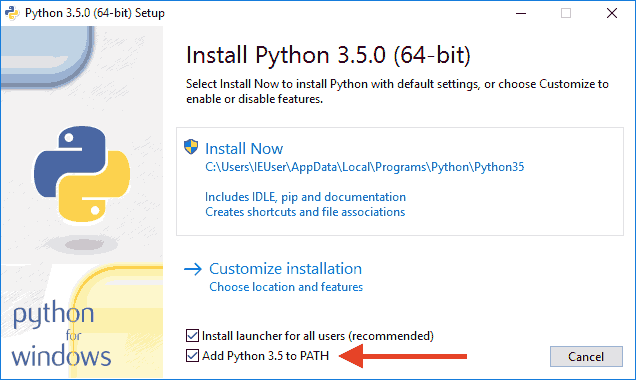
\includegraphics[width=0.6\linewidth]{fig/1048401552601344l.png}
\end{figure}


特别要注意勾上\texttt{Add\ Python\ 3.8\ to\ PATH},然后点 ``Install
Now'' 即可完成安装。

\hypertarget{ux8fd0ux884c-python}{%
\subsubsection{运行 Python}\label{ux8fd0ux884c-python}}

安装成功后,打开命令提示符窗口,敲入 python 后,会出现两种情况:

情况一:

\begin{pythoncode}
┌────────────────────────────────────────────────────────┐
│Command Prompt                                    - □ x │
├────────────────────────────────────────────────────────┤
│Microsoft Windows [Version 10.0.0]                      │
│(c) 2015 Microsoft Corporation. All rights reserved.    │
│                                                        │
│C:\> python                                             │
│Python 3.8.x ...                                        │
│[MSC v... 64 bit (AMD64)] on win32                      │
│Type "help", "copyright", "credits" or "license" for mor│
│information.                                            │
│>>> _                                                   │
│                                                        │
│                                                        │
└────────────────────────────────────────────────────────┘
\end{pythoncode}

看到上面的画面,就说明 Python 安装成功!

你看到提示符\texttt{\textgreater{}\textgreater{}\textgreater{}}就表示我们已经在
Python 交互式环境中了,可以输入任何 Python
代码,回车后会立刻得到执行结果。现在,输入\texttt{exit()}并回车,就可以退出
Python 交互式环境(直接关掉命令行窗口也可以)。

情况二:得到一个错误:

\begin{pythoncode}
┌────────────────────────────────────────────────────────┐
│Command Prompt                                    - □ x │
├────────────────────────────────────────────────────────┤
│Microsoft Windows [Version 10.0.0]                      │
│(c) 2015 Microsoft Corporation. All rights reserved.    │
│                                                        │
│C:\> python                                             │
│'python' is not recognized as an internal or external co│
│mmand, operable program or batch file.                  │
│                                                        │
│C:\> _                                                  │
│                                                        │
│                                                        │
│                                                        │
└────────────────────────────────────────────────────────┘
\end{pythoncode}

这是因为 Windows
会根据一个\texttt{Path}的环境变量设定的路径去查找\texttt{python.exe},如果没找到,就会报错。如果在安装时漏掉了勾选\texttt{Add\ Python\ 3.8\ to\ PATH},那就要手动把\texttt{python.exe}所在的路径添加到
Path 中。

如果你不知道怎么修改环境变量,建议把 Python
安装程序重新运行一遍,务必记得勾上\texttt{Add\ Python\ 3.8\ to\ PATH}。

\hypertarget{ux5c0fux7ed3}{%
\subsubsection{小结}\label{ux5c0fux7ed3}}

学会如何把 Python 安装到计算机中,并且熟练打开和退出 Python 交互式环境。

在 Windows 上运行 Python 时,请先启动命令行,然后运行\texttt{python}。

在 Mac 和 Linux 上运行 Python 时,请打开终端,然后运行\texttt{python3}。

